%!TEX root=../../../main.tex

Kravet til pH-proben er at den skal virke omgående når der hældes gødning i vandet. Dette vil sige at den skal omgående kunne fortælle systemet når der er den korrekte pH-værdi, når der doseres gødning. Efter nogle søgninger på Google blev der fundet frem til at en glasprobe var det meste effektive, men samtidig og så det billigste. 

\begin{figure}[H]
	\centering 
	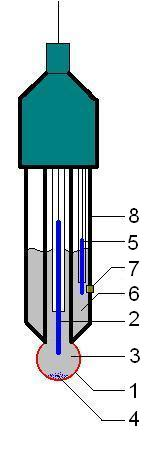
\includegraphics[scale=0.7]{HardwareArkitektur/Sensore/pH_probe_billeder/Glass_electrode_wiki.jpg}
	\caption{Tegning af en glasprobe. kilde: Wikipedia}
	\label{photo:pH-probe}
\end{figure}     

pH værdi er en måde at angive hvor mange hydrogen-ioner der er i væsken. Definitionen af en syre er at den modtager hydrogen-ionerne og definitionen af en base er at den afgiver hydrogen-ioner. Vand kan både optræde som en syre og en base, dette skyldes at vand vil modtage hydrogen-ionerne når der hældes en base i, men det vil afgive hydrogen-ioner når der hældes en syre i. På figur \ref{photo:pH-skala} ses at har vi $10^{-14}$ mol/l af H+ ioner har vi en pH-værdi på 14. 

 \begin{figure}[H]
	\centering 
	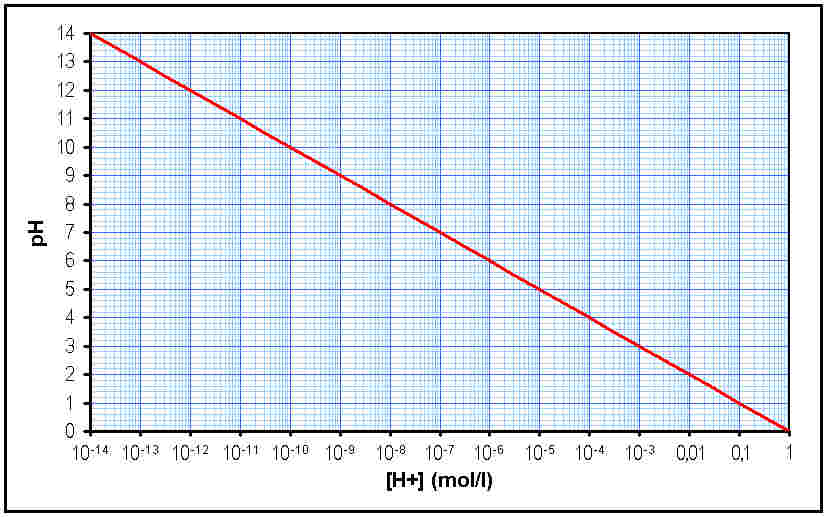
\includegraphics[scale=0.4]{HardwareArkitektur/Sensore/pH_probe_billeder/PH-skala.jpg}
	\caption{Graf over pH-værdi. kilde: Wikipedia}
	\label{photo:pH-skala}
\end{figure}   

Måden glasproben virker på at at den internt er fyldt op med saltsyre HCL. I figur \ref{photo:pH-probe} punkt 3 er koncentrationen $1*10^{-7}$ mol/l. I punkt 6 er koncentrationen $0.1$ mol/l. På denne måde bliver der genereret en spænding når der er et overskud eller underskud af H+ ioner på ydersiden af punkt 1. H+ ionerne vil tiltrække CL- ionerne som ses i punkt 4. Punkt 2 og 5 er elektroderne som vi måler spændingen over. I figur  \ref{photo:probeslope} ses outputtet fra proben i forhold til pH-værdien i den væske den er i. 

 \begin{figure}[H]
	\centering 
	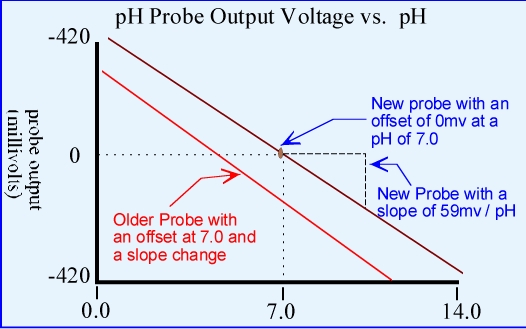
\includegraphics[scale=0.4]{HardwareArkitektur/Sensore/pH_probe_billeder/probeslope.jpg}
	\caption{Outputtet fra pH-proben}
	\label{photo:probeslope}
\end{figure} 

For at få en præcis måling af væsken kræver det at der laves en kaliberering af pH-proben en gang hver måned, da proben vil drifte med tiden. Det ses også på figur \ref{photo:probeslope} at en ny probe vil give en højrer spænding en en ældre. Dette betyder at den skal kalibreres en gang i mellem. Til kalibrering af proben skal der bruges noget buffervæske. En buffervæske er en væske med en præcis pH-værdi således at proben kan indstilles efter det. Måden vi vil gøre det på er ved at have en buffer med pH-værdi 7. Når systemet startes op skal proben kalibreres og der vil være en rød LED på karet der lyser. For at kalibrere proben sættes proben ned i buffervæsken og efter ca 30 sekunder trykkes der på en knap som sidder på karet og karet indlæser herved værdien til kalibrering. På figur \ref{photo:buffer_vaeske} ses at buffervæsken varierer sin pH-værdi ved temperaturforskelle. Dette vil også være gældende for andre væsker, dette er ikke noget vi tager højde for i vores målinger, men det burde blive implementeret i et salgsklart system. 

 \begin{figure}[H]
	\centering 
	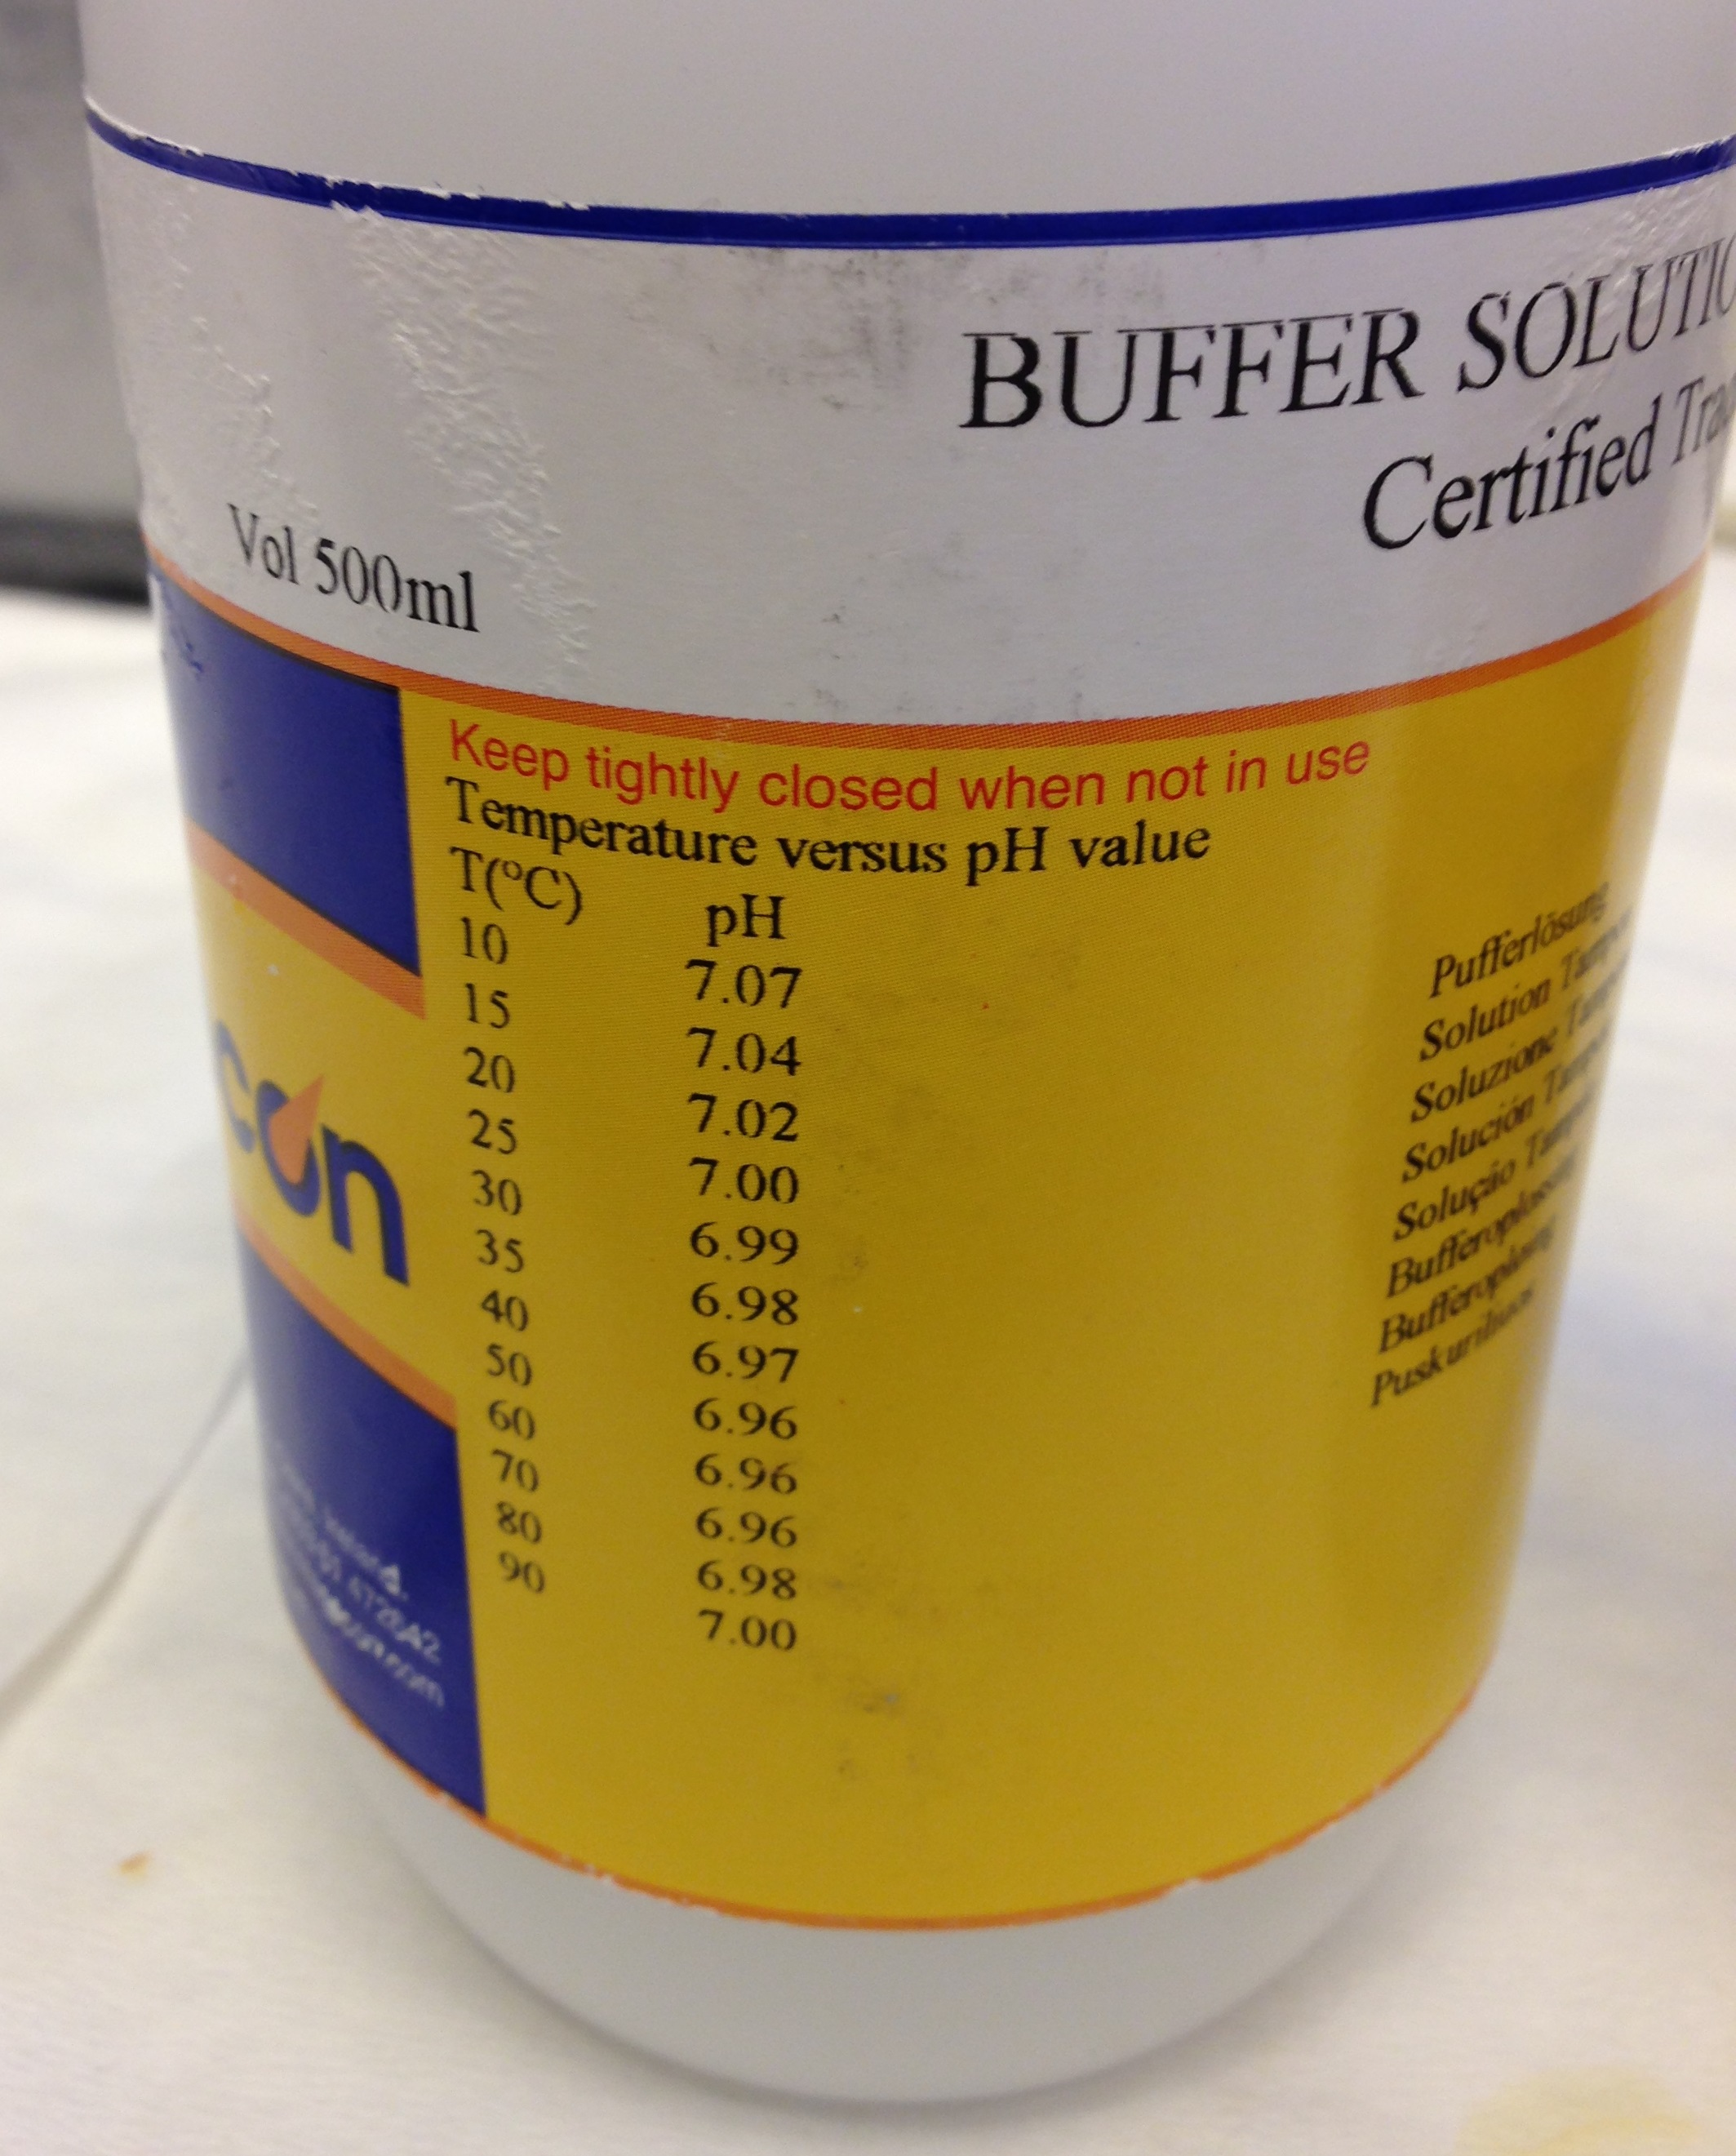
\includegraphics[scale=0.1]{HardwareArkitektur/Sensore/pH_probe_billeder/buffervaeske.jpg}
	\caption{Temperaturens indflydelse på pH-værdien i buffervæsken}
	\label{photo:buffer_vaeske}
\end{figure} 
Nedenfor ses koden til pH-proben. Koden er klar til at blive implementeret i kar-softwaren. Men for overskuelighedens skyld vælges det at vise den individuelle kode her. Der er oprettet en funktion getPhVal() som returnerer pH-værdien.

\lstinputlisting[language=c]{HardwareArkitektur/Sensore/kode/pH_kode.txt} 



